\section{Materials and methods}
\label{sec:method}

\subsection{Data}
\label{sub:data}
\begin{itemize}
	\item \textbf{MNIST dataset} \cite{MNIST}: i.i.d. images, $\vec{X} = \set{\vec{X}\order{i}}^N_{i=1}$, of handwritten digits:
	\begin{itemize}
		\item $28 \times 28$ pixels with one channel.
		\item \textbf{Training set} (including validation set) of 60000 images.
		\item \textbf{Test set} of 10000 images.
	\end{itemize}
	\item $\vec{x} = \vec{X}\order{i}$ for simplicity.
\end{itemize}

\subsection{Model}
\label{sub:the_model}

\begin{figure*}
	\centering
	\usetikzlibrary{positioning}
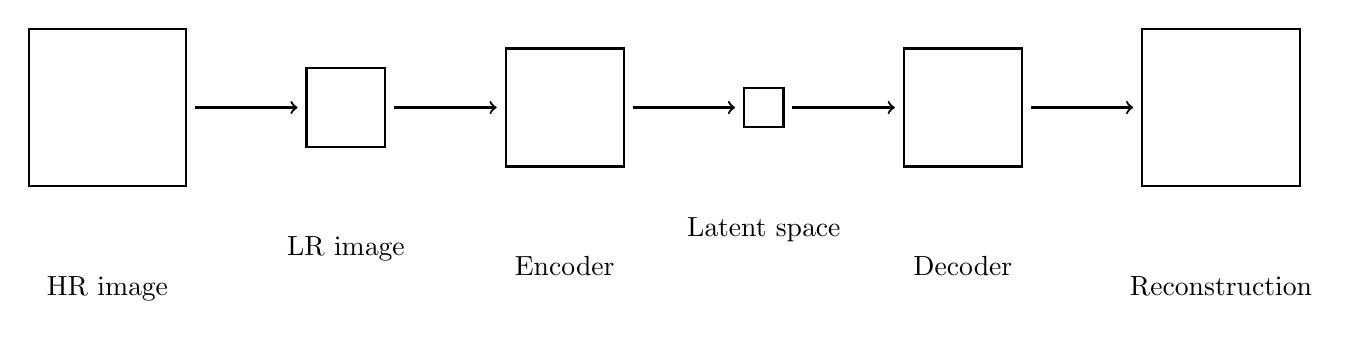
\begin{tikzpicture}[x = 1cm, y = 1cm, thick,
		image/.style={rectangle, draw, inner sep = 0pt, minimum size = 2 cm},
		network/.style={rectangle, draw, inner sep = 0pt, minimum size = 2 cm},
		arrow/.style={ ->, shorten <= 1 mm, shorten >= 1 mm}
	]
	
	\node[image, minimum size = 2 cm] (HR) at (0, 0) {};
	\node[below = of HR] {HR image};
	
	\node[image, minimum size = 1 cm, right = 1.5 cm of HR] (LR) {};
	\node[below = of LR] {LR image};
	
	\node[network, minimum size = 1.5 cm, right = 1.5 cm of LR] (encoder) {};
	\node[below = of encoder] {Encoder};
	
	\node[network, minimum size = 0.5 cm, right = 1.5 cm of encoder] (latent) {};
	\node[below = of latent] {Latent space};
	
	\node[network, minimum size = 1.5 cm, right = 1.5 cm of latent] (decoder) {};
	\node[below = of decoder] {Decoder};
	
	\node[image, minimum size = 2 cm, right = 1.5 cm of decoder] (reconstruction) {};
	\node[below = of reconstruction] {Reconstruction};
	
	\draw[arrow] (HR) -- (LR);
	\draw[arrow] (LR) -- (encoder);
	\draw[arrow] (encoder) -- (latent);
	\draw[arrow] (latent) -- (decoder);
	\draw[arrow] (decoder) -- (reconstruction);
	
\end{tikzpicture}

	\caption{Diagram of model. Originals, $\vec{x}\idx{HR}$, are binarised and downsampled, $\vec{x}\idx{LR}$. Reconstructions, $\tilde{\vec{x}}\idx{HR}$, are they results of the VAE.}
	\label{fig:diagram}
\end{figure*}

For the reconstruction of high-resolution (HR) digits from low-resolution (LR) digits in the MNIST dataset, our model assume the same underlying data generating process behind the production of digits to infer the same structure between them. Each variable in $\vec{X}$ are assumed to be drawn from a normal distribution\dots 
\change{Finish description of model. See method.tex in poster directory.}

\subsubsection{Preprocessing of HR images}
\label{ssub:downsampling}

\begin{itemize}
	\item Binarised using Bernoulli sampling.
	\change{Mention robustness to variations because of this.}
	\item Downsampled by a factor of $d$ using \textbf{mean filter} (pooling layer).
\end{itemize}

\subsubsection{Variational auto-encoder}
\label{ssub:vae}

Using mean-field variational Bayes \cite{Kingma2013}, we build a generative model with an approximated decoding posterior distribution, $\enc{\vec{z}|\vec{X}}$ mapping the observed variables $\vec{X}$ into the unobserved latent variables $\vec{z}$. The generative part of the model is then using the conditional likelihood $\dec{\vec{X},\vec{z}}$ to redo the probabilistic process of producing a digit pixel for pixel. \\  
The model is trained based on a per-pixel loss-function derived from the marginal log-likelihood of each datapoint, $i$:
\begin{equation}
	\log \dec{\vec{X}} = \log \dec{\vec{X}\order{1}, ..., \vec{X}\order{N}} = \sum^N_{i=1} \log \dec{\vec{X}\order{i}} 
\end{equation}
From now on we denote $\vec{X}\order{i} = \vec{x}$ for shorter and uncluttered notation.
The marginal log-likelihood can be decomposed like for the EM-algorithm and variational inference \cite[\S10.2]{Bishop2006}:
\begin{equation}
	\log \dec{\vec{X}\order{i}} = D_{KL}\left( \enc{\vec{z}|\vec{x}}||\dec{\vec{z}|\vec{x}}\right) + \mathcal{L}\left(\vec{\theta},\vec{\phi};\vec{x}\right)
\end{equation} 
Here the first term is the Kullback-Leibler divergence, which is a non-negative entropy measure of how much the 2 distributions differ.
\begin{equation}
	D_{KL}\left( \enc{\vec{z}|\vec{x}}||\dec{\vec{z}|\vec{x}}\right) = \int \enc{\vec{z}|\vec{x}} \log \curlies*{ \frac{\dec{\vec{x}|\vec{z}}}{\enc{\vec{z}|\vec{x}} } } \D{\vec{z}}
\end{equation}

Since the KL-divergence is non-negative the second term (``free energy'') works as a variational lower bound and follows the inequality:

\begin{gather}
	\begin{split}
		\log \dec{\vec{x}} & \ge \mathcal{L}\left(\vec{\theta},\vec{\phi};\vec{x}\right)
		\\ & =
		\int \enc{\vec{z}|\vec{x}} \log \curlies*{ \frac{\dec{\vec{x},\vec{z}}}{\enc{\vec{z}|\vec{x}} } } \D{\vec{z}} \\ 
		& = \E_{\enc{\vec{z}|\vec{x}}} \brackets{- \log \enc{\vec{z}|\vec{x}} + \log \dec{\vec{x},\vec{z}} } 
		\\
		& = -D_{KL}\parens{ \enc{\vec{z}|\vec{x}}||\dec{\vec{z}} } 
		\\ 
		& \quad+ \E_{\enc{\vec{z}|\vec{x}}} \brackets{\log \dec{\vec{x}|\vec{z}} }   	
	\end{split} 
\end{gather}

Maximizing $\mathcal{L}$ wrt. the model parameters, $\phi$ and $\theta$, thereby minimizes the $D_{KL}\left( \enc{\vec{z}|\vec{x}}||\dec{\vec{z}|\vec{x}}\right)$ bringing the. When $D_{KL}\rightarrow 0$ the approximated variational distribution $\enc{\vec{z}|\vec{x}}\rightarrow \dec{\vec{z}|\vec{x}}$.

\change{Write that the VAE reduces to a normal auto-encoder when $D_{KL}\left( \enc{\vec{z}|\vec{x}}||\dec{\vec{z}|\vec{x}}\right)$ is left out.}

\change{Write about differences in distribution for continuous (Gaussian) and binary (Bernoulli) data.}

\change{Write about the Stochastic Gradient Variational Bayes method in short.}

\change{Write that output is the mean of the Bernouilli distribution.}

% Differentiation of L
% Reparameretization trick
% Output parameters (mu and sigma)

% TODO: Add algorithm from Kingma13: Algorithm 1 Minibatch version of the Auto-Encoding VB (AEVB) algorithm.

\subsection{Experiments}
\label{sub:experiments}

\change{Write as text and clarify choices for each hyperparameter.}

\begin{itemize}
	\item Reconstruct HR images using the VAE for different values of latent size $N_{\vec{z}}$ and downsampling factor $d$. The encoder and decoder consists of two \textbf{fully-connected neural networks} with $200$ hidden neurones each and \textbf{rectifying activation functions}. $L = 1$ for the sampling of $\vec{z}$ as Kingma et al \cite{Kingma2013}.
	\change{Add batch size.}
	\item Compare reconstructions using VAE with a bicubic interpolation upscaling.
\end{itemize}
